\chapter{Introducción}
\label{introduccion}

\section{Objetivo}
El propósito principal de este Trabajo Final de Grado (TFG) es profundizar en el conocimiento del funcionamiento de un campo solar de concentradores cilindroparabólicos (CCP) mediante el desarrollo de una herramienta de simulación programada en Python 3. Para ello, se ha partido del modelo teórico desarrolado en su Tesis Doctoral por el profesor de la Universidad Nacional de Educación a Distancia (UNED), el Dr.~Rubén Barbero Fresno y se ha empleado una metodología basada en el paradigma de la programación orientada a objetos (POO). El desarrolo de este trabajo ha supuesto un reto personal por la necesidad de adquirir habilidades en el manejo de diferentes herramientas antes desconocidas para mí, como el lenguaje de programación Python 3 y sus diferentes librerías para el cálculo científico (Numpy) y el tratamiento de datos (Pandas). Finalmente, todo el código se encuentra publicado y accesible a través de GitHub y se puede interactuar con la versión final del código de simulación a través de un Notebook Jupyter.

Los resutaldos obtenidos son compatibles con los datos de generación de un campo solar real dentro de las limitaciones que los diferentes modos de operación y eventos impredecibles (paradas de planta para mantenimiento, disparos por avería, etc\ldots{}) introducen en el proceso. En este proyecto solo se aborda la simulación del sistema del campo solar, el único sistema dentro del alcance del modelo teórico de partida. Para la simulación de planta sería necesario el desarrollo de
modelos para gran número de sistemas como por ejemplo, los generadores de vapor, almacenamiento térmico, turbina, sistemas auxiliares de bombeo, sistemas de tratamiento de agua, torre de refrigeración, etc\ldots{} No obstante, la metodología seguida permite que en el futuro este proyecto pueda ser ampliado de forma sistemática con la incoroporación de nuevas clases de objetos que aprovechen los métodos de entrada y salida ya programados para interactuar con ellos. En todo caso, se han empleado valores de rendimientos estimados para los principales subsistemas de planta con el fin de ofrecer una estimación de la energía eléctrica finalmente vertida a la red.

\section{Estructura de la memoria}
Esta memoria se estructura en 5 capítulos y un anexo con el código fuente.

En este primer capítulo se describen los objetivos del TFG y se ofrece una introducción a las características de los concentradores cilindroparabólicos. 
El segúndo capítulo presenta el modelo teórico de partida y se detallan las ecuaciones que describen los sistemas que más adelante serán modelados.
El tercer capítulo aborda el modelado de los diferentes sistemas necesarios para la caracterización del campo solar. Se procede a la validación por comparación con otra herramienta de simulación y se presentan los resultados de algunos análisis paramétricos.
En el cuarto capítulo se aborda una análisis del funcionamiento de una central solar termoeléctrica y se contratastan los resultados de la simulación del campo solar con los datos reales disponibles.
Finalmente, en el quinto capítulo se presentan algunas conclusiones y propuestas de desarrollo futuro.

\section{Concentradores cilindroparabólicos}

Existen principalmente cuatro tecnologías para el aprovechamiento de la radiación solar directa en sistemas térmicos: concentrador cilindro-parabólico CCP, central de torre, concentrador Fresnel y disco parabólico. La tecnología de central de torre y la de CCP son las que cuentan en la actualidad con una mayor madurez y gran número de centrales en operación y en construcción en todo el mundo \cite{islamComprehensiveReviewStateoftheart2018}. En España actualmente hay medio centenar de centrales CCP en operación \cite{Protermosolar}, alguna de ellas desde hace más de una década, quedando probado que el estado del arte y la madurez de la tecnología garantizan el correcto funcionamiento del sistema. Este tipo de sistema presenta un alto grado de replicabilidad, modularidad y aprovechamiento del terreno. Desde el punto de vista económico, esta tecnología también resulta muy favorable ya que los costes de inversión y operación han sido comercialmente probados, al menos, para los sistemas termoeléctricos.

\begin{figure}
 \centering
  \subfloat[Central Solar de Torre. Fuente \cite{Protermosolar}]{
   \label{f:torre}
    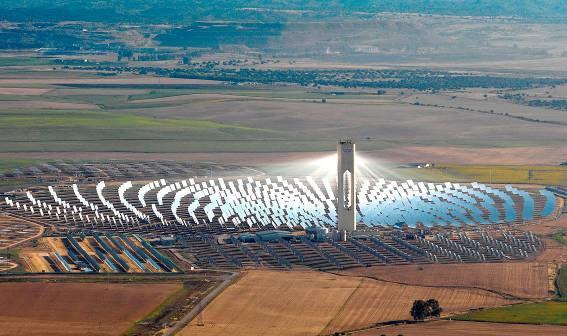
\includegraphics[width=0.5\textwidth]{images/torre.png}}
  \subfloat[Concentradores de Disco Parabólico. Fuente \cite{Protermosolar}]{
   \label{f:disco}
    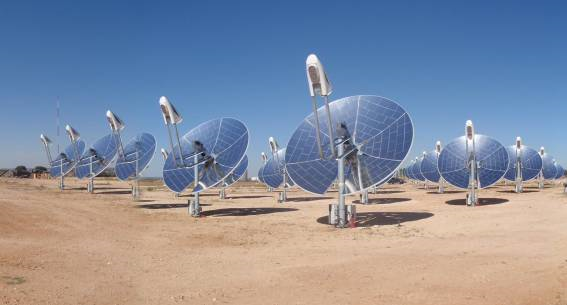
\includegraphics[width=0.5\textwidth]{images/disco.png}}
  \\
   \subfloat[Colector Cilindro-Parabólico. Fuente: Propia]{
   \label{f:ccp}
    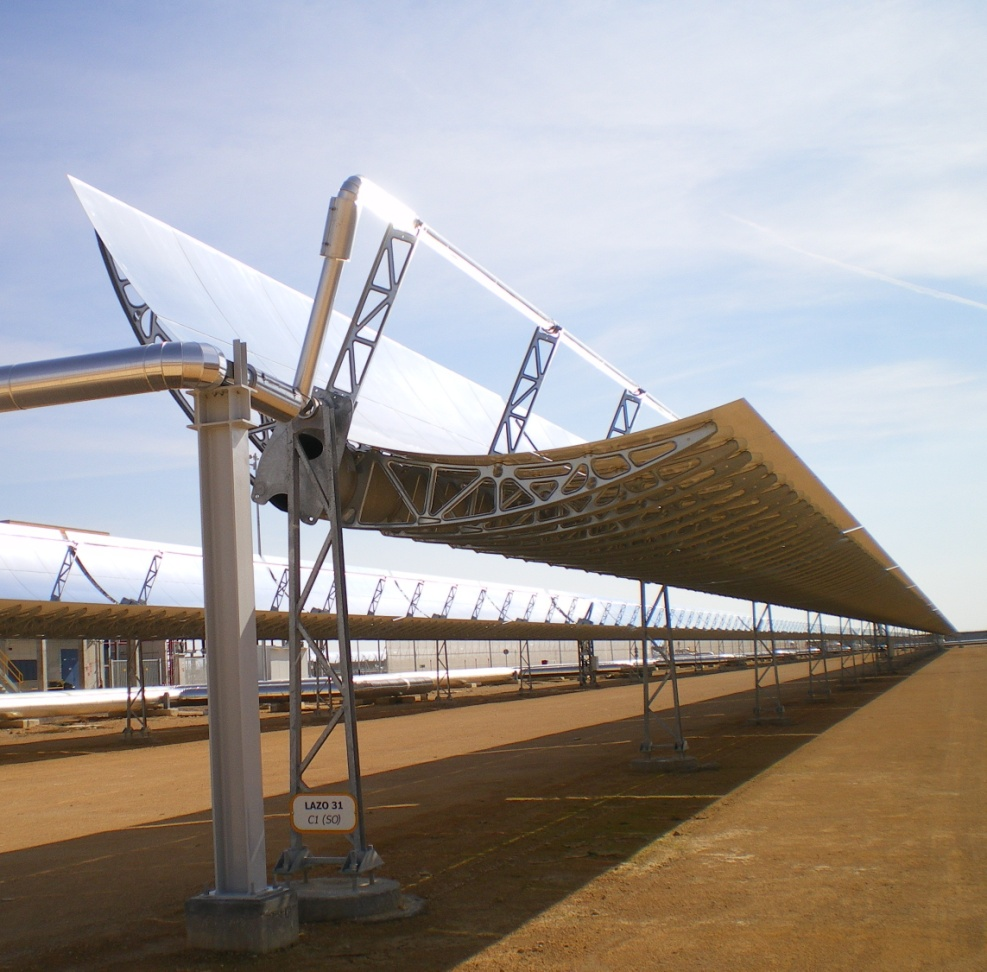
\includegraphics[width=0.5\textwidth]{images/ccp.png}}
   \subfloat[Concentrador de tipo Fresnel. Fuente \cite{Protermosolar}]{
   \label{f:fresnel}
    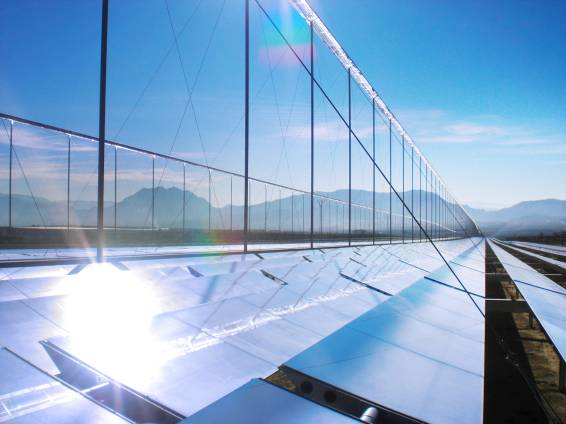
\includegraphics[width=0.5\textwidth]{images/fresnel.png}}
 \caption{Tecnologías solares de concentración}
 \label{f:tecnologias_concentracion}
\end{figure}


En un CCP pueden distinguirse cuatro elementos principales: el reflector o concentrador, el tubo absorbedor, el sistema de seguimiento y el fluido caloportador.

\subsection{El concentrador cilindroparabólico}
\label{concentrador}
Un CCP consiste en una superfice a modo canal  de sección parabólica que refleja la radiación solar directa concentrándola sobre un tubo absorbedor colocado en la línea focal del paraboloide. Dentro de los diferentes sistemas de concentración solar pertenece al grupo de los concentradores lineales, al igual que los sistemas de concentración tipo Fresnel y al contrario que los sistemas de concentración de torre central o de discos parabólicos, en cuyo caso estaríamos hablando de sistemas de concentración puntuales. Por el tubo absorbedor se puede hacer circular algún fluido que se calentará debido a la radiación incidente sobre el tubo.  Se trata de una transformación directa de energía luminosa en energía térmica con una buena eficiencia y que puede alcanzar temperaturas de hasta 675 K.

\begin{figure}
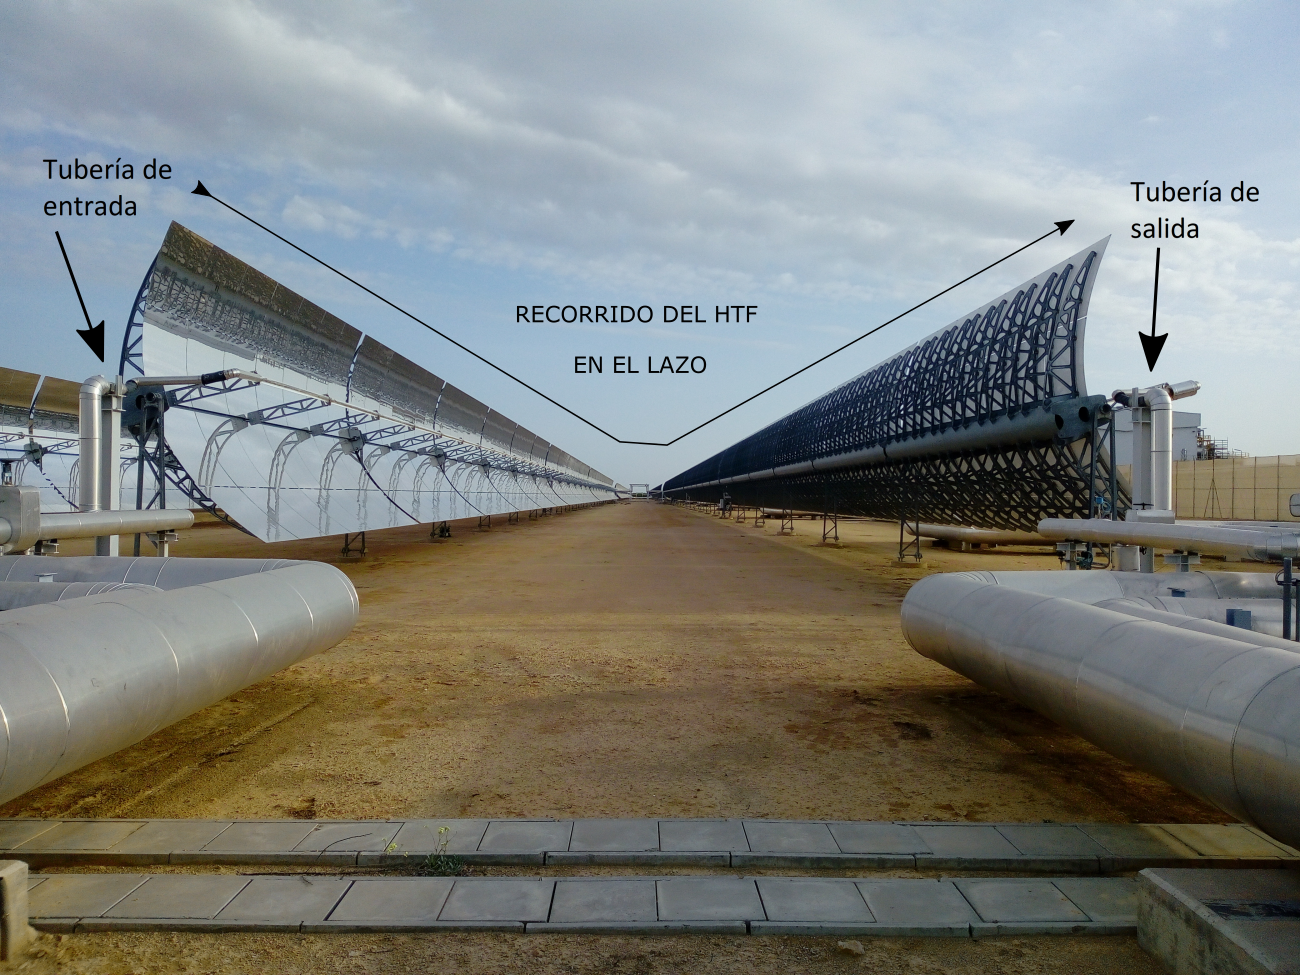
\includegraphics[width=0.9\linewidth]{images/entrada_salida_lazo2_texto.png}
\caption{Perspectiva de un lazo completo. Se indica el sentido del recorrido del HTF en el lazo, desde la tubería de entrada hasta la de salida. Fuente: Propia} 
\label{fig:entrada_salida_lazo}
\end{figure}


\begin{figure}
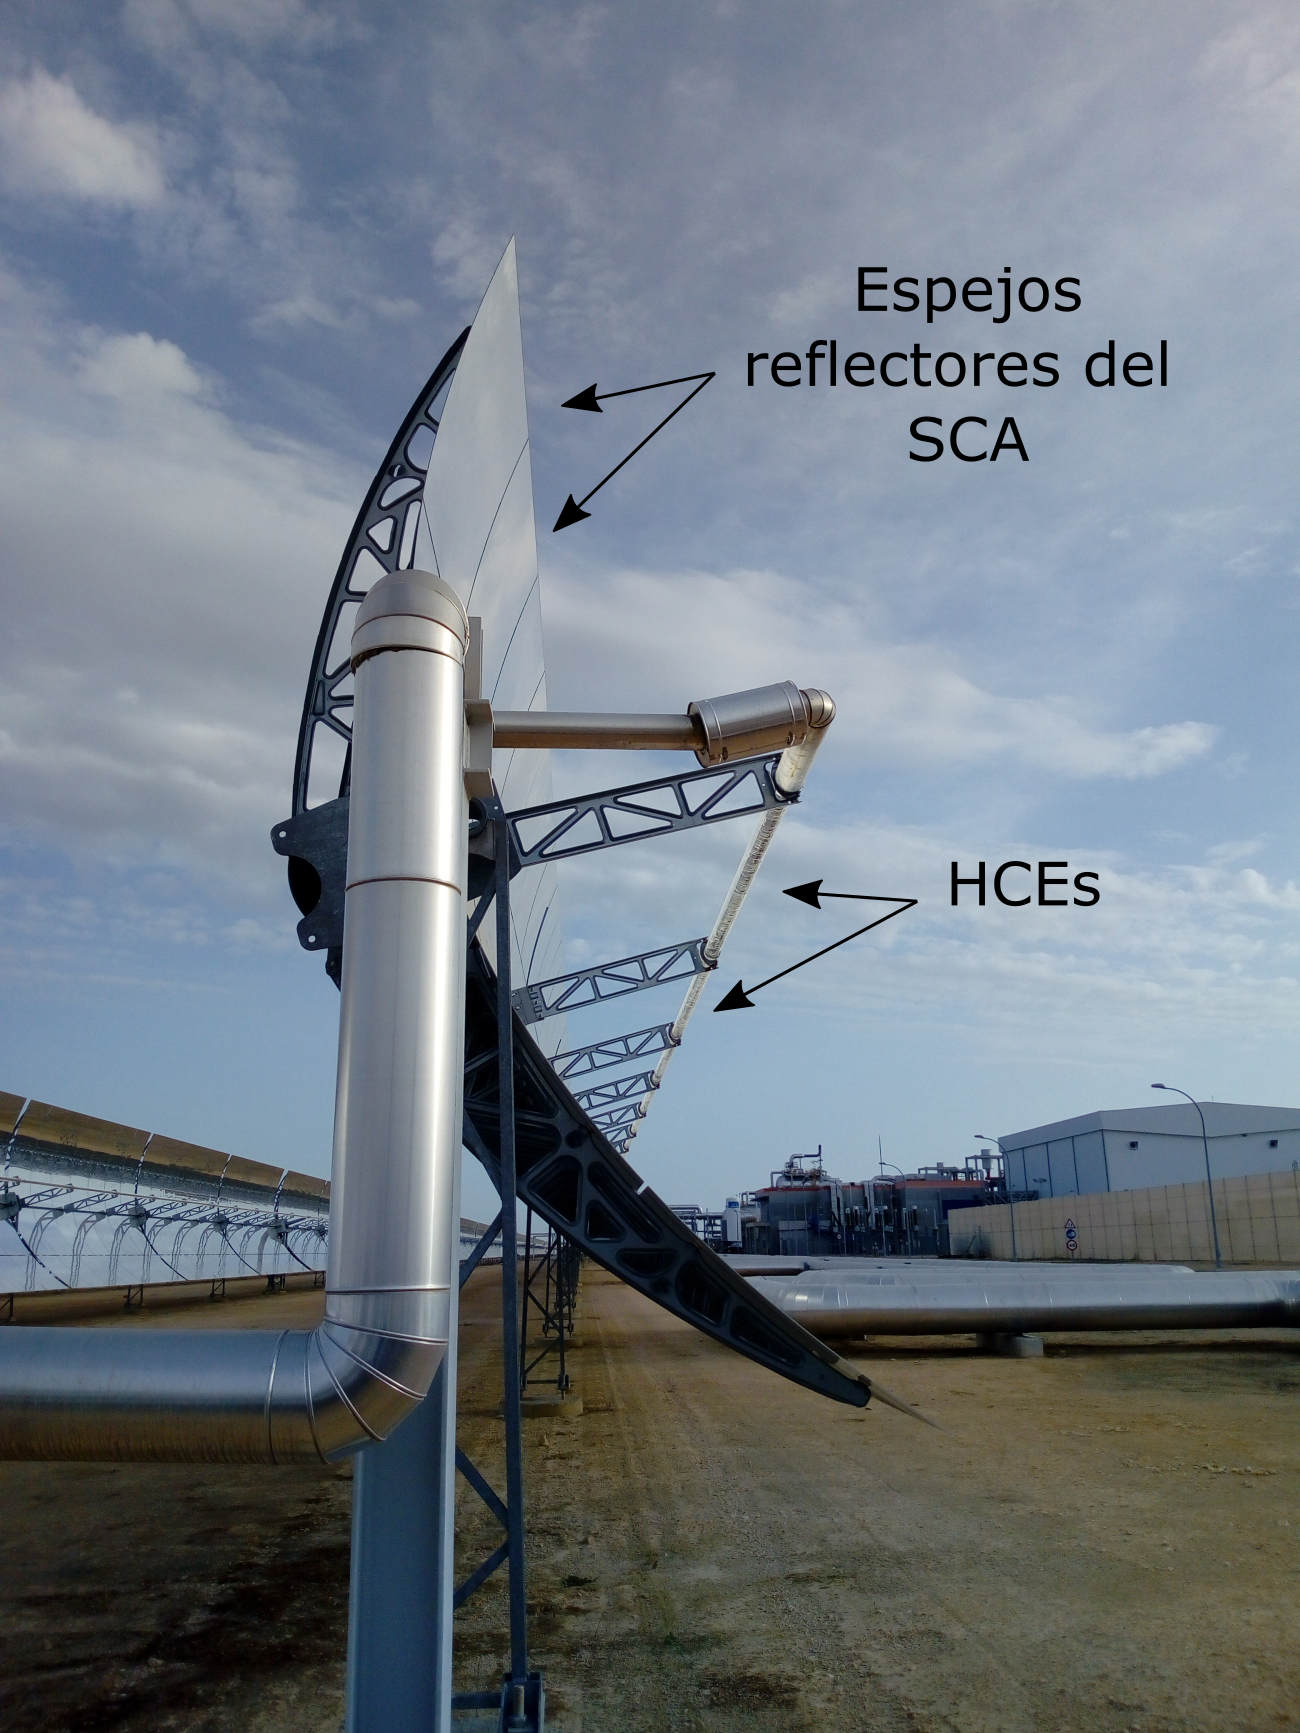
\includegraphics[width=0.9\linewidth]{images/perfil_sca_2_texto.png}
\caption{Vista de perfeil de un SCA. Pueden distinguirse algunos HCEs y los brazos de soporte. Fuente: Propia} 
\label{fig:perfil_sca}
\end{figure}

\subsection{El tubo absorbedor o receptor}
\label{tuboabsorbedor}
A lo largo del eje focal del concentrador se instala una conducción por la que circula un fluido caloportador o transmisor del calor (HTF por sus siglas en ingles, Heat Transfer Fluid). Esta conducción está compuesta en realidad por una serie de elentos tubulares denominados Heat Collector Element, HCE. Los HCE consisten en tubo de acero con una envolvente de vidrio de tal forma que en el proceso de fabricación se ha dejado extraido el aire que queda entre ambos (region anular o annulus). De esta forma se reducen las pérdidas de calor por convección a través de la región anular. La soldadura vidrio-metal y unos elementos denominados getters que absorben, hasta cierto punto, algunas moléculas que puedan filtrarse a la región anular durnte la vida de operacion del HCE permiten que éste cuente con pérdidas reducias de calor mientras no se produzca la rotura del vidrio o la saturación de dichos getters. 

\subsection{El sistema de seguimiento}
\label{sistemadeseguimiento}
Para que se produzca la concentración de la radiación solar incidente ésta debe ser perpendicular al eje que pasa por el foco y la base de la parábola. La primera consecuenca es que solo puede aprovecharse plenamente la componente normal de la radiación solar incidente (DNI). Dado que el Sol varía su posición relativa al concentrador continuamente, el conjunto reflector-tubo absorbedor está montado sobre una estructura que pueda girar sobre un eje con el fin de segir la trayectoria solar a lo largo del día. Salvo instalaciones especiales en laboratorios, no se emplean seguidores a dos ejes pues la complejidad de los colectores con movimiento basado en dos ejes es tal que no permite su rentabilidad debido a los costes de mantenimiento. Por tanto, el sistema de seguimiento más empleado consiste en mover la estructura del colector con un grado de libertad en torno a un eje que, en las plantas solares cuyo objetivo es maximizar el vertido anual de energía eléctrica a la red, cuenta con una orientación Norte-Sur, lo cual lleva a que exista una importante diferencia entre la generación en los meses de verano y los meses de invierno, siendo mayor en los primeros. Si lo que se persigue es obtener una producción más estable a lo largo del año, la orientación más adecuda del eje sería Este-Oeste.

La rotación del colector requiere un mecanismo de accionamiento, eléctrico o hidráulico,
dependiendo en muchos casos de las dimensiones y el peso de los elementos del colector. Para abaratar costes se suele emplear un mismo mecanismo para mover varios módulos.

El control del movimiento se puede llevar a cabo de forma autónoma, en el propio colector, dotándolo de algún dispositivo para detectar la posición del Sol en el cielo. Otra opción es emplear algoritmos matemáticos que calculan la posición del Sol para cada momento del día, en cualquier día del año. Una vez calculada la posición solar, se mueve el colector hasta colocarlo correctamente orientado. Este método requiere algún sistema para conocer la posición exacta del colector. Lo normal es emplear un codificador angular.
Dado que el colector solar se encuentra en movimiento, las conexiones del tubo absorbedor con las tuberías de entrada y salida de éste deben permitir el giro en los puntos de unión. Para esto se emplean conexiones flexibles y juntas rotativas combinadas adecuadamente. El coste de estos elementos es también elevado por lo que la elección de una configuración adecuada puede suponer un importante ahorro de costes en la instalación y el mantenimiento.

\subsection{El fluido caloportador}
\label{fluidocaloportador}

El rango de temperatura ideal para trabajar con colectores cilindro parabólicos es de 425 K a 675 K.
Para temperaturas superiores las pérdidas térmicas son altas y para temperaturas inferiores hay otros
colectores más económicos (colectores de placa plana y colectores de tubo de vacío).
El tipo de fluido a emplear depende de la temperatura de trabajo. El agua desmineralizada es una
buena opción para temperaturas inferiores a los 450 K. A mayor temperatura es preferible el aceite
sintético debido a que no aumenta tanto su presión. Nosotros emplearemos aceite sintético
Santotherm VP-1. Este aceite puede trabajar bien hasta los 672 K pero tiene un punto de
congelación de 285 K. Para nosotros no supondrá un problema dado que podremos emplear un
sistema de apoyo auxiliar para mantener el aceite recirculando a una temperatura adecuada cuando
la radiación solar no permita sobrepasar esta temperatura de congelación.
